\chapter{Explications techniques}
\label{sec:technique}

%% CONTIKI =================================================================
\section{Contiki}

	Afin de créer notre sonde, nous avons utilisé Contiki, notamment la Pile réseau IPv6 et les buffers cycliques.
	
	\subsection{Pile réseau de Contiki}
	
		Contiki possède trois piles réseau :
		\begin{itemize}
			\item Rime
			\item IPv4
			\item IPv6
		\end{itemize}
		Bien évidemment, celle qui nous intéresse ici est la pile IPv6. 
		
		\subsubsection{Organisation de la pile IPv6}
			
			L'implémentation de la pile réseau nous permet d'utiliser les communications avec aisance. C'est grâce à elle que nous pouvons envoyer et recevoir des messages.
			
			La pile réseau se découpe en quatre couches :
			\begin{itemize}
				\item Couche réseau
				\item Couche MAC -- Medium Access Control
				\item Couche RDC -- Radio Duty Cycling
				\item Couche radio
			\end{itemize}
			
			\clearpage
			
			\begin{figure}[htp]
				\centering
				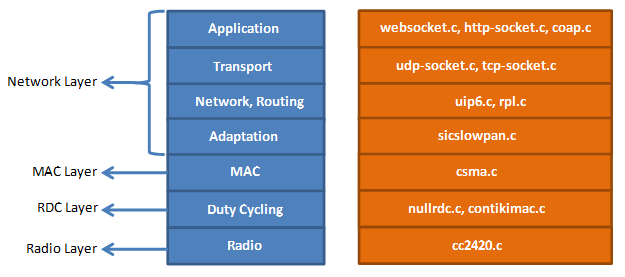
\includegraphics[width=16cm]{images/Contikinetstack}
				\caption{Organisation de la pile réseau de Contiki.}
				\label{fig:contikinetstack}
			\end{figure}
			
		\subsubsection{Packetbuf}
		
			Pour envoyer et recevoir des paquets, Contiki se base sur un buffer unique de paquets -- paquetbuf, qu'ils soient entrants ou sortants.
			Le buffer est découpé en deux parties, la première pour l'en-tête, et la deuxième pour les données.
			
			\begin{figure}[htp]
				\centering
				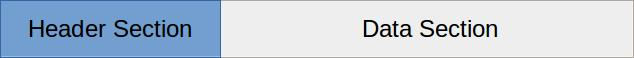
\includegraphics[width=12cm]{images/Buf.jpg}
				\caption{Découpage du buffer de paquets de Contiki.}
				\label{fig:buf}
			\end{figure}
			
			Une différence est faite entre les paquets sortants et les paquets entrants.
			
			\clearpage
			\begin{figure}[htp]
				\centering
				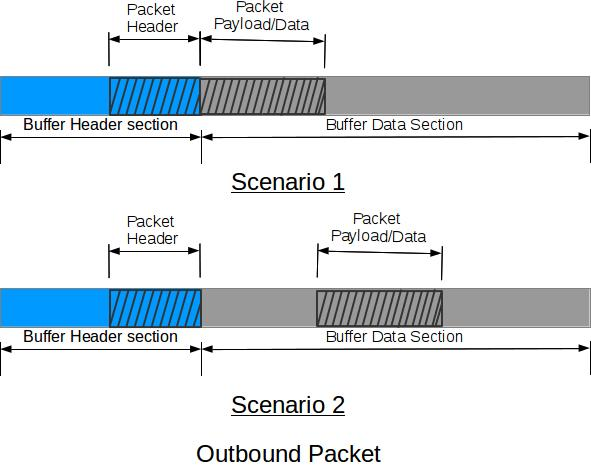
\includegraphics[width=13cm]{images/Out.jpg}
				\caption{Répartition des données pour un paquet sortant.}
				\label{fig:outbuf}
			\end{figure}
			
			
			Le buffer pour les paquets sortants permet de construire ce qu'on veut envoyer de façon structurée, avec une séparation de l'en-tête et des données qui permet de modifier l'un sans influer sur l'autre. \\
			Ce découpage donne accès aux attributs des paquets, ce qui comprend 4 niveaux d'utilisations :
			\begin{itemize}
				\item Local
				\item Entre deux voisins
				\item Entre les noeuds en bout de la communication
				\item L'expéditeur et le receveur locaux, et l'expéditeur et le receveur finaux
			\end{itemize}
			Ces attributs sont toutes les informations utiles à la diffusion et au routage du paquet, par exemple le canal, le numéro de séquence, le nombre de sauts, et bien d'autres, 26 au total.
			
			\clearpage
			
			\begin{figure}[htp]
				\centering
				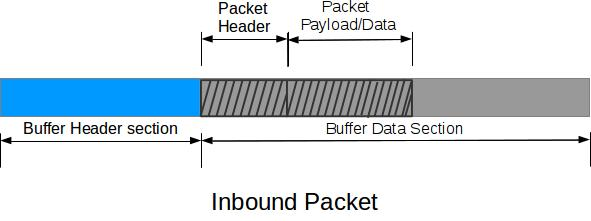
\includegraphics[width=13cm]{images/In.jpg}
				\caption{Répartition des données pour un paquet entrant.}
				\label{fig:inbuf}
			\end{figure}
			
			Le buffer pour les paquets entrant ne fait pas la différence entre en-tête et données, et met tout dans la partie données. Cela permet d'économiser de la puissance de calcul en évitant d'interpréter l'en-tête.\\
			Les fonctions à disposition permettent uniquement de récupérer le paquet brut. Pour effectuer nos vérifications, ils nous faut donc étudier la construction des paquets.
	
	\subsection{Systèmes de stockage Contiki}
		
		Pour nos vérifications superficielles, il nous a été demandé de stocker temporairement quelques informations à propos des paquets du trafic. Nous avons considéré plusieurs options pour stocker ces informations.

		\subsubsection{Contiki Coffee file system}
%			\begin{itemize}
%				\item Expliquer comment écrire dedans
			Contiki possède plusieurs systèmes de fichiers qui implémentent l'interface de Contiki File System, dont Coffee. Coffee est utilisé sur les appareils équipés avec de la mémoire flash ou de l'EEPROM. Contiki s'occupe de l'implémentation matérielle, et Coffee fournit une API qui est similaire aux opérations sur les fichiers du langage C standard.\\
			
%				\item Expliquer pourquoi on ne l'a pas utilisé
			L'intérêt d'un système de fichier est d'envoyer d'un seul coup plusieurs données, afin de limiter le nombre de transmissions, et donc de consommer moins d'énergie. Aussi, garder les données en mémoire de façon locale permet, en cas de transmission échouée, de ne pas les perdre définitivement.
			
			Nous avons préféré nous tourner vers la mémoire volatile pour enregistrer les informations, pour avoir une solution moins lourde.
%			\end{itemize}
		\subsubsection{Volatile}
			
			La mémoire volatile de Contiki peut s'utiliser de plusieurs façons :\\ \\
			\textbf{Listes}\\
%			\begin{itemize}
%				\item Expliquer comment écrire dedans
				La librairie de Contiki pour les listes procure une liste chaînée dans laquelle les informations souhaitées sont stockées puis récupérées par la suite. La librairie est utilisée partout dans Contiki pour stocker les listes des processus, les files de paquets, les listes des voisins, et d'autres tables.\\
				\begin{figure}[htp]
					\centering
					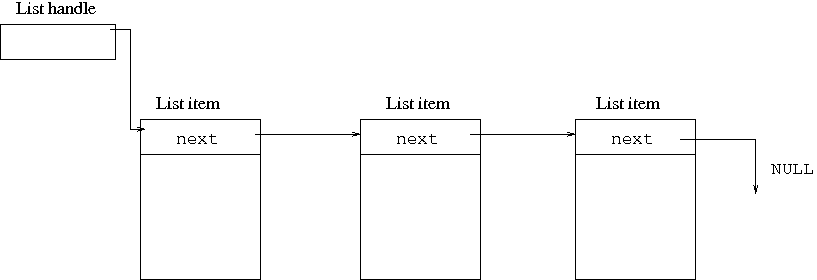
\includegraphics[width=16cm]{images/linked-list}
					\caption{Architecture d'une liste chaînée sur Contiki.}
					\label{fig:list}
				\end{figure}
				Les objets de la liste sont des structures qui sont définies par le module qui utilise la liste. La seule condition est que le premier objet de la liste doit être un pointeur, qui est utilisé par la librairie pour lier les objets ensemble dans la liste.\\
				Une liste de Contiki consiste d'un pointeur et de zéro ou plus objets dans la liste, comme montré dans l'illustration ci-dessus. Le pointeur pointe vers le premier objet de la liste.\\
				
				La liste était l'une des solutions potentielles à notre besoin de stockage, mais il a été décidé de faire appel à un moyen encore plus léger : le buffer cyclique.
%				\item Expliquer pourquoi on ne l'a pas utilisé
%			\end{itemize}
			\clearpage
			\textbf{Buffers cycliques}\\
%			\begin{itemize}
%				\item Expliquer comment écrire dedans
				Il y a plusieurs endroits dans Contiki où un gestionnaire d'interruption doit garder des données qui peuvent être indépendamment être lues par d'autres parties de Contiki. Le gestionnaire et les fonctions de lectures doivent être synchronisées pour éviter les problèmes de concurrence, parce le gestionnaire peut préempter les parties qui lisent les données à n'importe quel moment. Les mécanismes de lecture et d'écriture sont donc pensées pour être indépendantes de chacune.\\
				\begin{figure}[htp]
					\centering
					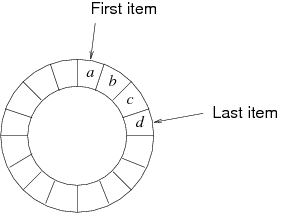
\includegraphics[width=10cm]{images/ringbuf}
					\caption{Architecture d'un buffer cyclique sur Contiki.}
					\label{fig:ringbuf}
				\end{figure}\\
%				\item Expliquer pourquoi on l'a utilisé
%			\end{itemize}
				Ci-dessus : Un buffer cyclique avec quatre objets, a, b, c et d. L'objet a est le prochain à sortir du buffer. Le d est l'objet le plus récemment inséré. Le premier et dernier pointeur permettent d'y accéder respectivement.\\\\
				Un buffer cyclique ( parfois appelé buffer en anneau ) est une structure de données qui garde les données en mémoire sous la forme d'un anneau comme montré ci-dessus. Les données sont stockées dans le buffer, et sont lues dans le même ordre que celui dans lequel elles ont été insérées. La structure est donc proche d'une FIFO ( First In First Out ) ou file en français.\\
				Contiki propose une librairie qui implémente les buffers cycliques, qui garde en mémoire des octets dans un tableau dont la taille doit être une puissance de deux, inférieure ou égale à 256. La raison pour la contrainte sur les puissances de deux est que la structure implémente les fonctions sur les pointeurs de début et de fin avec des opérateurs booléens.\\
				Aussi, la taille maximale de 256 octets est là pour permettre à ces pointeurs de début et de fin de tenir dans une structure de 8 bits. L'octet habituel est la seule structure de donnée qui peut être mise à jour de façon atomique, ce qui est important pour assurer la synchronisation entre les lectures et écritures sur le buffer cyclique, même si l'un préempte l'autre.\\
				
				Malgré les contraintes imposées par cette structure, sa légèreté et ses propriétés de synchronisation sont des gros avantages sur les autres structures : Les paquets n'attendent pas que Contiki ait fini d'écrire dans sa mémoire.
	
%% 6LoWPAN =================================================================
\section{6LoWPAN}
	\subsection{Compression des headers}
%		\begin{itemize}
%			\item Pourquoi compresser ?
		Comme évoqué dans l'analyse de l'existant, les communications via IPv6 se révèlent peu pratiques pour des systèmes contraints, surtout à cause des headers ( ou entêtes ) trop volumineux qui réduisent la charge utile de données contenues par un paquet, multipliant le nombre de paquets. \\
		La RFC 4944 définit LOWPAN\_HC1, le mécanisme de compression des en-têtes IPv6 pour les LowPAN. Elle intègre aussi la compression de l'en-tête UDP sur 4 octets, mais n'autorise pas la compression du Checksum. De plus, elle restreint la plage des ports UDP de 61616 à 61631 afin de compresser à 4 bits cette valeur.
		
		\begin{figure}[htp]
			\centering
			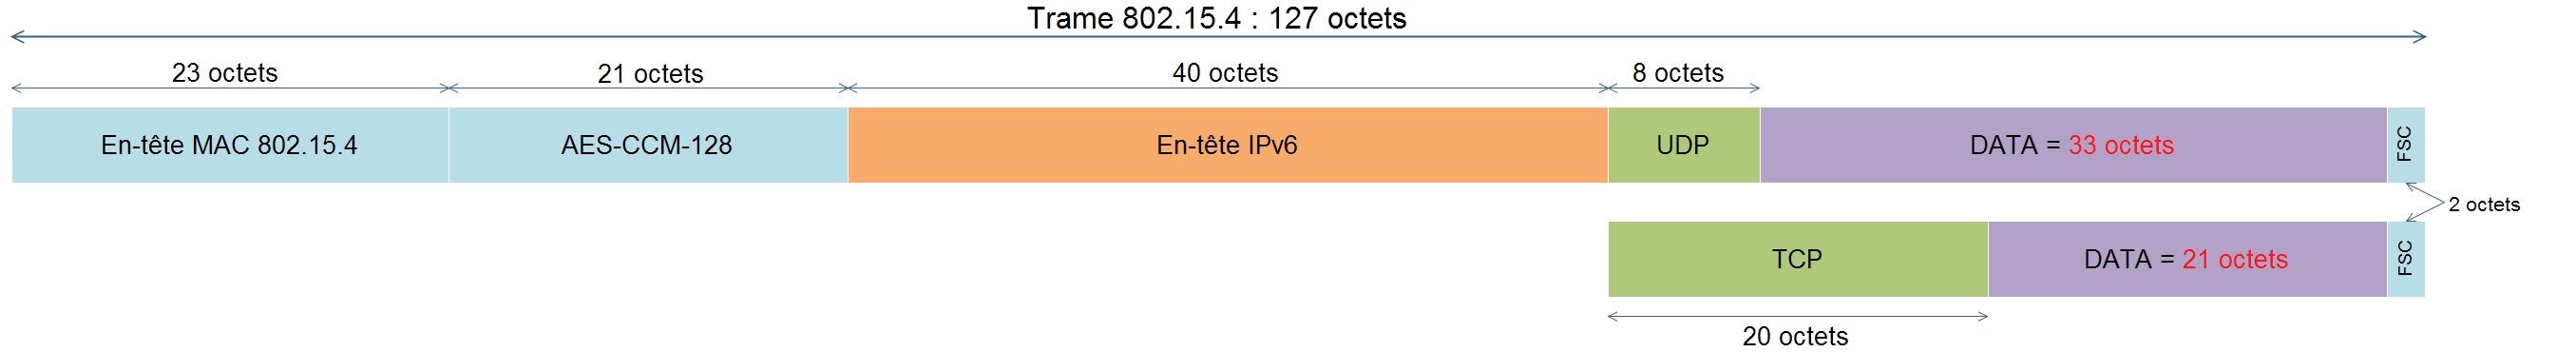
\includegraphics[width=16cm]{images/TramePasComp.jpg}
			\caption{Trame IPv6 non compressée.}
			\label{fig:tramepascomp}
		\end{figure}
		
		\begin{figure}[htp]
			\centering
			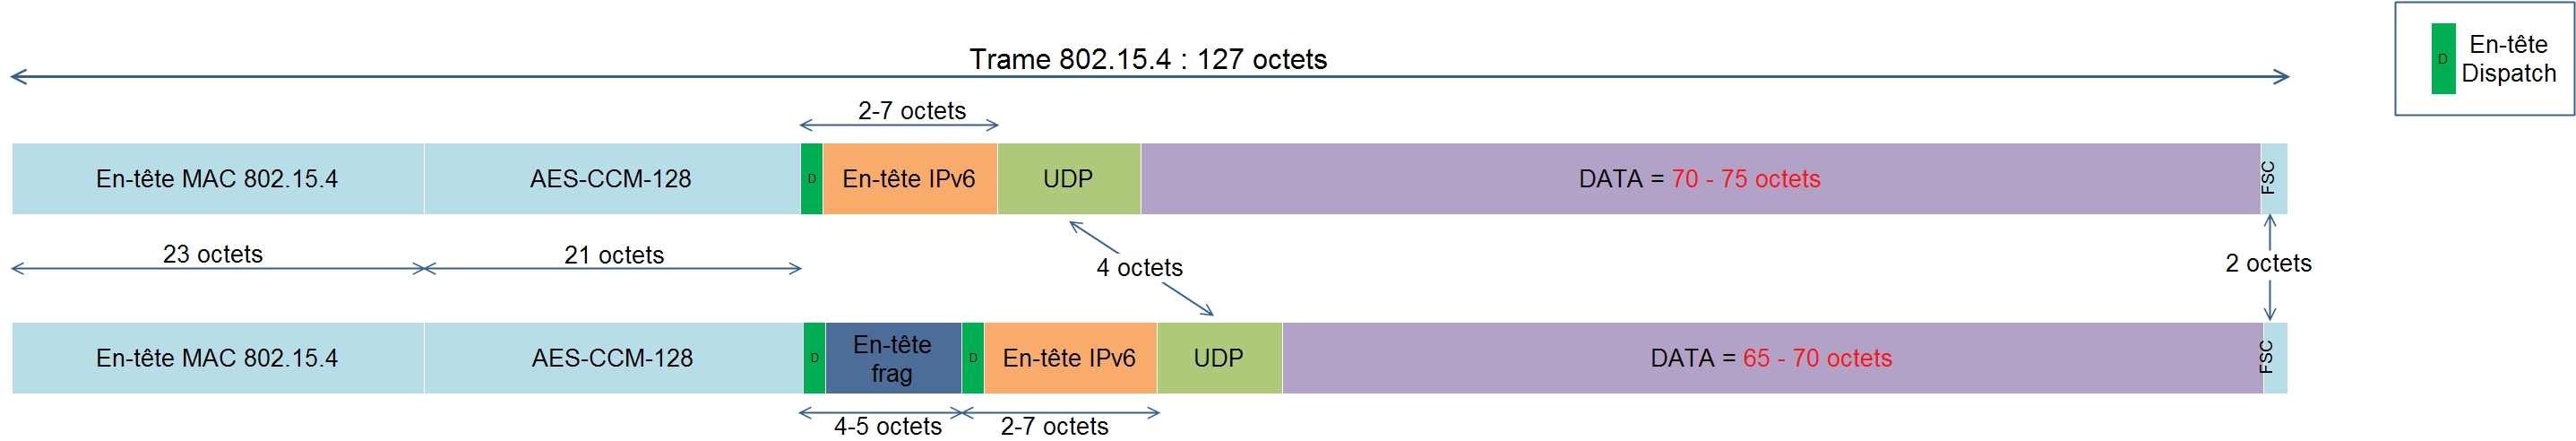
\includegraphics[width=17cm]{images/TrameComp.jpg}
			\caption{Trame IPv6 compressée.}
			\label{fig:tramecomp}
		\end{figure}
		On remarque que la charge utile est doublée grâce à la compression d'en-tête.
%			\item Comment ça marche ( avec images )
%		\end{itemize}
%	
	\subsection{Attaques possibles}
		Notre but étant de travailler vers la sécurisation d'un réseau 6LoWPAN, nous avons étudié différentes attaques possibles sur ce type de réseau. Elles se classent en deux catégories : Celles qui sont pertinentes pour notre sujet, et celles qui ne le sont pas.\\
		
		\subsubsection{Non-pertinentes}
%	\begin{itemize}
%		\item Qui nous intéressent pas directement
%		\begin{itemize}
%			\item Attaques passives ( écoute )
%			\item Brouillage des ondes
%			\item Inondation de paquets
%		\end{itemize}
			Les attaques passives telles que les écoutes, les attaques de brouillage des ondes, ou d'inondation de paquets sont difficilement repérables par un noeud du réseau. Ces attaques ne sont donc pas pertinentes dans le cadre de notre sujet, car il faudrait fait usage de matériel différent de nos capteurs.
		\subsubsection{Pertinentes}
%		\item Qui nous intéressent
%		\begin{itemize}
%			\item Spoofing
%			\item Paquets dupliqués
%			\item Paquets fabriqués
%			\item Sybil attack
%		\end{itemize}
			D'autres attaques, comme la duplication ou falsification de paquets, le spoofing et l'attaque Sybil sont des exemples que nous avons étudié pour préparer des vérifications sur notre capteur.\\
			
			La \textbf{falsification} de paquets peut entrainer une nombre de situations d'attaque, tout en étant difficile à détecter. Un paquet peut être falsifié sur plusieurs champs ou un seul, pour avoir différents effets.\\
			Le \textbf{spoofing} est la situation où un attaquant envoie un paquet en falsifiant l'adresse source pour se faire passer pour quelqu'un d'autre, généralement une adresse de confiance.\\
			La \textbf{duplication} de paquets est une autre manière de mener une attaque contre un réseau, par exemple, en renvoyant un message d'authentification antérieur.\\
			L'\textbf{attaque Sybil} est particulière, il s'agit d'un seul acteur possédant plusieurs identités, par exemple un seul noeud qui envoie des messages avec deux ou plus adresses sources qui n'étaient pas utilisées auparavant. C'est ce qui la différencie d'un simple spoof.
%	\end{itemize}
%	Nos possibles solutions du coup


%%% Local Variables: 
%%% mode: latex
%%% TeX-master: "isae-report-template"
%%% End: 
